\documentclass{article}

% Language setting
% Replace `english' with e.g. `spanish' to change the document language
\usepackage[english]{babel}

% Set page size and margins
% Replace `letterpaper' with `a4paper' for UK/EU standard size
\usepackage[letterpaper,top=2cm,bottom=2cm,left=3cm,right=3cm,marginparwidth=1.75cm]{geometry}

% Useful packages
\usepackage{xeCJK}
\usepackage{amsmath}
\usepackage{amssymb}
\usepackage{graphicx}
\usepackage{caption}
\usepackage{float}
\usepackage[colorlinks=true, allcolors=blue]{hyperref}
\usepackage{appendix}
\usepackage{listings}
\usepackage{xcolor}

\setCJKmainfont{SimSun}

% 自定义关键词格式
\newcommand{\keywords}[1]{\textbf{关键词:} #1}

\lstset{
    language=Python,
    basicstyle=\ttfamily\footnotesize,
    keywordstyle=\color{blue}\bfseries,
    stringstyle=\color{red},
    commentstyle=\color{gray}\itshape,
    numbers=left,
    numberstyle=\tiny\color{gray},
    stepnumber=1,
    numbersep=10pt,
    frame=single,
    breaklines=true,
    breakatwhitespace=false,
    showspaces=false,
    showtabs=false,
    tabsize=4,
    captionpos=b
}

% 设置图片和表格标题为中文
\captionsetup[figure]{name=图}
\captionsetup[table]{name=表}

\title{初探混合高斯分布}
\author{周陈序(523120910191)}

\begin{document}
\maketitle

\renewcommand{\abstractname}{摘要} % 更改摘要标题为中文
\begin{abstract}

本文以混合高斯分布为研究对象,通过理论推导和数值实验,系统分析了其分布特性及参数对分布形态的影响。针对混合高斯分布,本文首先定义并绘制其频率分布直方图,深入探讨了各参数(如 \(\mu_1\)、\(\sigma_1^2\)、\(\mu_2\)、\(\sigma_2^2\) 及 \(p\))对分布中“峰”特征的作用机制。随后,构造并分析了统计量 \( U \),研究样本量 \( n \) 对其频率分布直方图的影响。实验结果显示,随着 \( n \) 的增加,分布形态逐渐趋于正态,验证了中心极限定理的作用。

本文还通过矩母函数推导和数值模拟,深入解释了混合高斯分布的多峰特性及其演化规律。本研究不仅加深了对混合高斯分布的理论理解,也进一步展示了概率论在复杂分布分析中的实际应用价值,为后续的学习和研究奠定了基础。

\end{abstract}

\keywords{概率论,混合高斯分布,矩母函数,频率直方图,中心极限定理}

\newpage
\tableofcontents
\newpage

\section{引言}

概率论作为数学的重要分支,为我们提供了一个严密而系统的理论框架,用于描述和分析随机现象的本质及其规律。在实际应用中,概率论已广泛渗透到数据科学、机器学习、经济学、工程和自然科学等诸多领域,为理解不确定性提供了坚实的基础。

本次大作业以混合高斯分布为核心研究对象,通过探索其频率分布直方图、参数影响以及统计量的行为特性,旨在加深对概率论基本概念和方法的理解,并将理论知识融会贯通于实际问题的解决中。混合高斯分布作为一种重要的概率模型,因其灵活性和强大的拟合能力,在数据聚类、模式识别和信号处理等领域具有广泛的应用价值。本作业不仅涵盖了混合高斯分布的基本性质,还对其在复杂环境下的行为进行系统化分析。

通过分析频率分布直方图以及参数对分布特征的影响,探讨了混合高斯分布在不同条件下的表现;同时,通过构造特定统计量 \( U \),研究了样本量对其分布形态的影响,并利用矩母函数理论进行理论分析。这一过程充分体现了概率论理论与实践的结合,也进一步挖掘了混合高斯分布的统计特性和现实意义。


\section{任务一}

\subsection{混合高斯分布的定义}

随机变量$X \sim \mathcal{N}(\mu_1,\sigma_1^2)$,$Y \sim \mathcal{N}(\mu_2,\sigma_2^2)$,则$Z=X+\eta*Y$服从的分布称为混合高斯分布,其中$P(\eta=0)=p$,$P(\eta=1)=1-p$,$p \in [0,1]$。

\subsection{不同参数下混合高斯分布频率分布直方图及参数对频率分布直方图中“峰”的影响}

由上文定义可知,混合高斯分布的参数共有五个,分别为$\mu_1$,$\sigma_1^2$,$\mu_2$,$\sigma_2^2$以及$\eta$,本文设定$\mu_1=0$,$\sigma_1^2=1$,$\mu_2=5$,$\sigma_2^2=2$,$p=0.4$绘制出如图\ref{图:混合高斯分布}所示的混合高斯分布频率分布直方图,此处固定$X$服从标准正态分布,便于后续进一步探索不同参数对混合高斯分布“峰”的影响。

\begin{figure}[H]
\centering
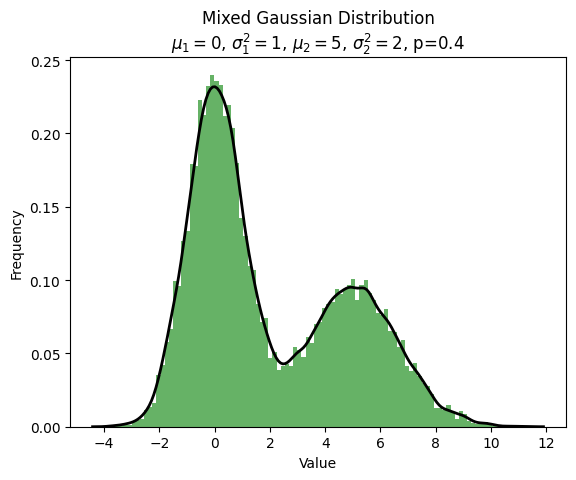
\includegraphics[width=0.5\linewidth]{figure/混合高斯分布.png}
\caption{\label{图:混合高斯分布}混合高斯分布($\mu_1=0$,$\sigma_1^2=1$,$\mu_2=5$,$\sigma_2^2=2$,$p=0.4$)}
\end{figure}

% 使用 \texorpdfstring 来避免警告
\subsubsection{\texorpdfstring{$\mu_2$对“峰”的影响}{mu2对“峰”的影响}}

下面本文将固定$\mu_1$,$\sigma_1^2$,$\sigma_2^2$,$p$,尝试设定不同的$\mu_2$以分析$\mu_2$对混合高斯分布“峰”的影响。为行文方便,下文每张图片对应的参数均已标注在图中,同时下文将用"主峰"代指由变量$X$生成的峰,用"次峰"代指由变量$Y$生成的峰。

首先,分别绘制$\mu_2=5$与$\mu_2=-5$的频率分布直方图,如图\ref{图:mu_2=5}和图\ref{图:mu_2=-5}所示。

\begin{figure}[H]
    \centering
    % 第一张图片
    \begin{minipage}[b]{0.4\linewidth}  % 控制第一张图片的宽度
        \centering
        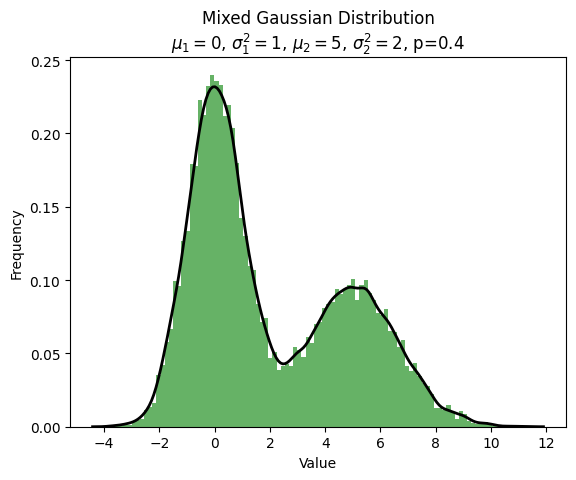
\includegraphics[width=\linewidth]{figure/混合高斯分布.png}  % 替换为图片路径
        \caption{\label{图:mu_2=5}}$\mu_2=5$
    \end{minipage}
    \hfill  % 两张图片之间的间隔
    % 第二张图片
    \begin{minipage}[b]{0.4\linewidth}  % 控制第二张图片的宽度
        \centering
        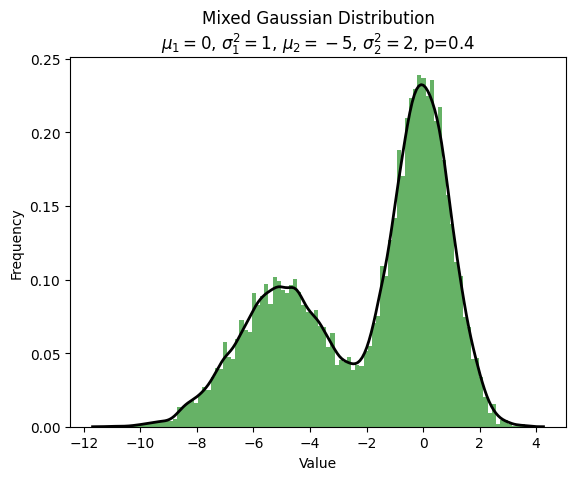
\includegraphics[width=\linewidth]{figure/mu_2=-5.png}  % 替换为图片路径
        \caption{\label{图:mu_2=-5}}$\mu_2=-5$
    \end{minipage}
\end{figure}

通过观察两张频率分布直方图,可以得出如下结论:当 $\mu_2$ 关于 $\mu_1$ 对称时,混合高斯分布的“峰”呈现对称性。通过改变其他参数并绘制相应的直方图(如图\ref{fig:对称}所示,包含了三组不同参数下的频率分布直方图),发现当 $\mu_1 = 0$ 时,只要保持 $\mu_2$ 关于 $\mu_1$ 的对称性,得到的直方图均表现出对称的“峰”特征,上述结论在$\mu_1 = 0$时的稳健性得到检验。然而,当 $\mu_1 \neq 0$ 时,尽管保持 $\mu_2$ 关于 $\mu_1$ 对称,直方图中的“峰”在相对位置上大致对称,但两峰之间会出现明显的“挤压”现象,导致图形的对称性破缺。随着 $\mu_1$ 的增大,这种对称性逐渐减弱。因此,可以推测,只有在特殊情况下,即 $\mu_1 = 0$ 时,混合高斯分布才具有显著的对称性。\label{sec:symmetry}

\begin{figure}[H]
    \centering
    \begin{minipage}[b]{0.3\linewidth}
        \centering
        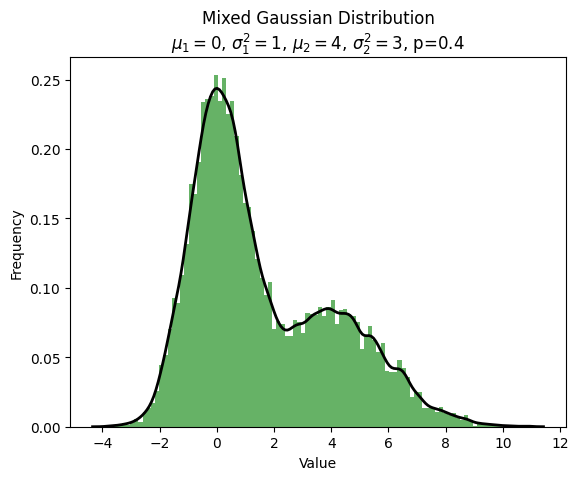
\includegraphics[width=\linewidth]{figure/对称1.png}
        \caption{对称1-1}
    \end{minipage}
    \hfill
    \begin{minipage}[b]{0.3\linewidth}
        \centering
        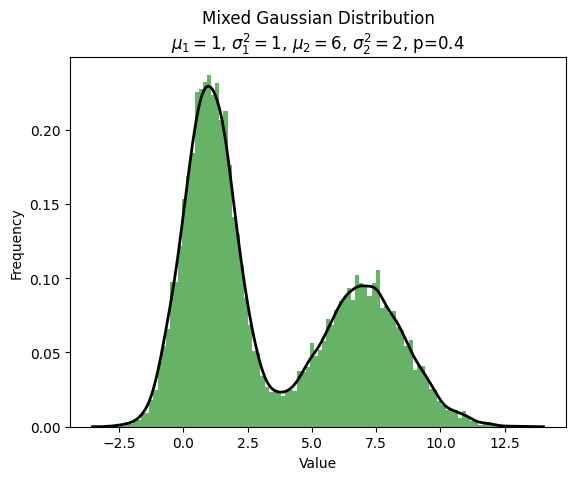
\includegraphics[width=\linewidth]{figure/对称3.png}
        \caption{对称2-1}
    \end{minipage}
    \hfill
    \begin{minipage}[b]{0.3\linewidth}
        \centering
        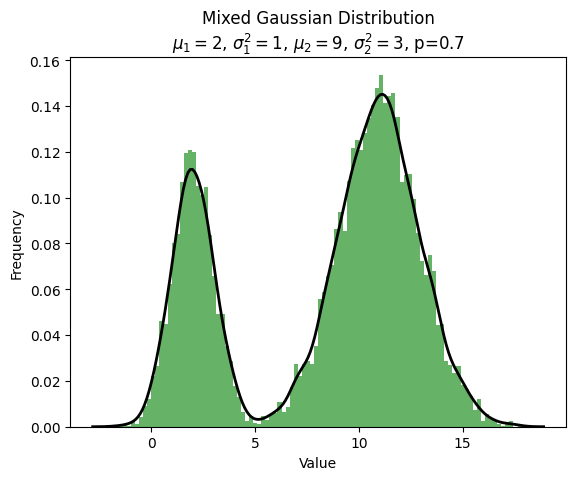
\includegraphics[width=\linewidth]{figure/对称5.png}
        \caption{对称3-1}
    \end{minipage}
    \hfill
    \vspace{4mm} % 控制上下图片间的间隔
    \begin{minipage}[b]{0.3\linewidth}
        \centering
        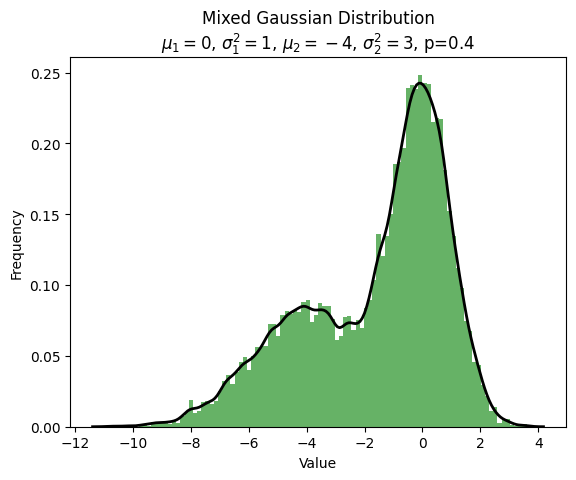
\includegraphics[width=\linewidth]{figure/对称2.png}
        \caption{对称1-2}
    \end{minipage}
    \begin{minipage}[b]{0.3\linewidth}
        \centering
        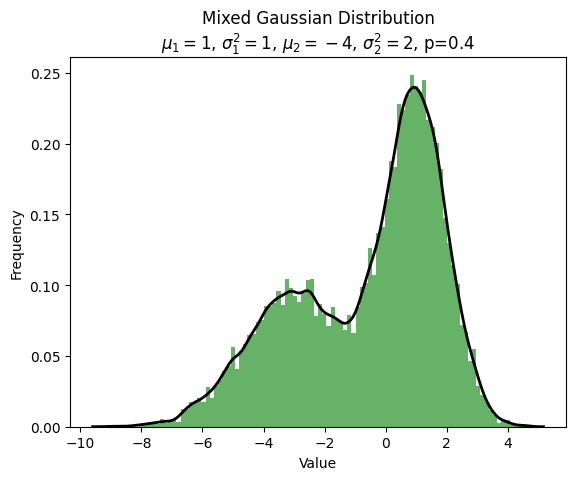
\includegraphics[width=\linewidth]{figure/对称4.png}
        \caption{对称2-2}
    \end{minipage}
    \hfill
    \begin{minipage}[b]{0.3\linewidth}
        \centering
        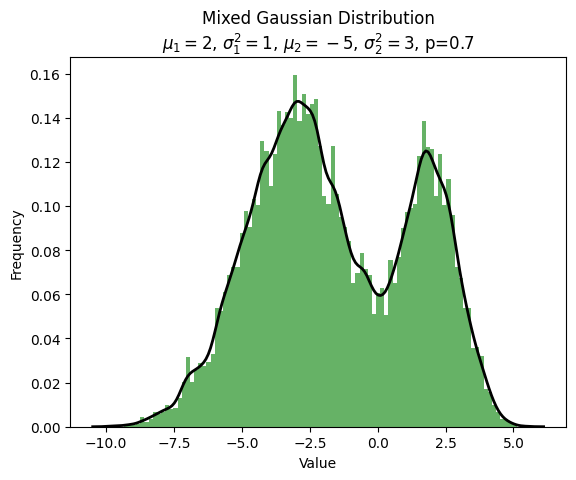
\includegraphics[width=\linewidth]{figure/对称6.png}
        \caption{对称3-2}
    \end{minipage}
    \caption{对称性探索}
    \label{fig:对称}
\end{figure}

本文从$\mu_2 = -6$开始,逐步增大$\mu_2$的值,绘制了对应的图像(图\ref{fig:mu_2递增})。通过观察“峰”的演变规律,可以得出以下结论:当$\mu_2$接近$\mu_1$时,图像中仅出现一个显著的主峰;然而,随着$\mu_2$与$\mu_1$之间的差距增大,次峰逐渐显现。进一步分析发现,主峰和次峰之间的距离随着$\mu_2$与$\mu_1$差距的增大而逐步扩大,推测该距离的变化主要由$\mu_2$的取值所决定。\label{sec:peak_dist}

\begin{figure}[H]
    \centering
    \begin{minipage}[b]{0.2\linewidth}
        \centering
        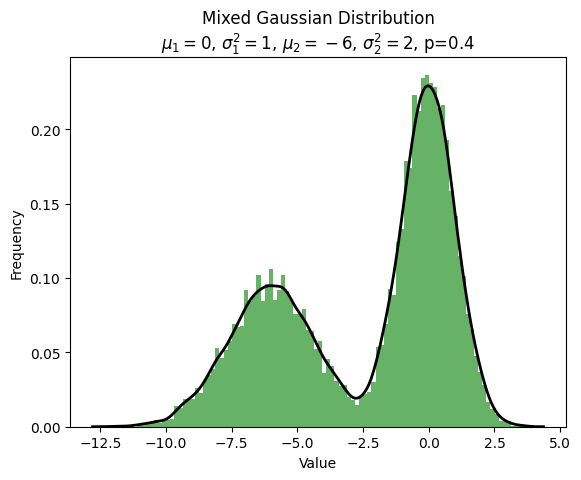
\includegraphics[width=\linewidth]{figure/mu_2=-6.png}
        \caption{$\mu_2=-6$}
    \end{minipage}
    \hfill
    \begin{minipage}[b]{0.2\linewidth}
        \centering
        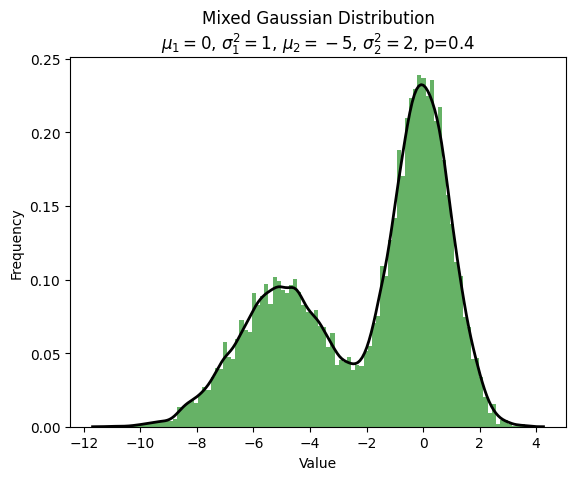
\includegraphics[width=\linewidth]{figure/mu_2=-5.png}
        \caption{$\mu_2=-5$}
    \end{minipage}
    \hfill
    \begin{minipage}[b]{0.2\linewidth}
        \centering
        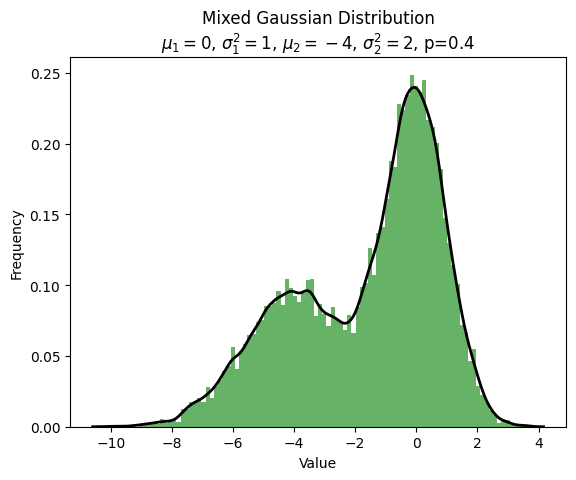
\includegraphics[width=\linewidth]{figure/mu_2=-4.png}
        \caption{$\mu_2=-4$}
    \end{minipage}
    \hfill
    \begin{minipage}[b]{0.2\linewidth}
        \centering
        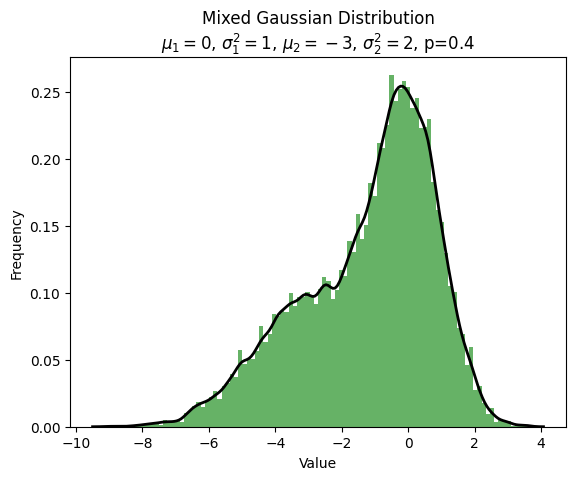
\includegraphics[width=\linewidth]{figure/mu_2=-3.png}
        \caption{$\mu_2=-3$}
    \end{minipage}
    \vspace{4mm} % 控制上下图片间的间隔
    \begin{minipage}[b]{0.2\linewidth}
        \centering
        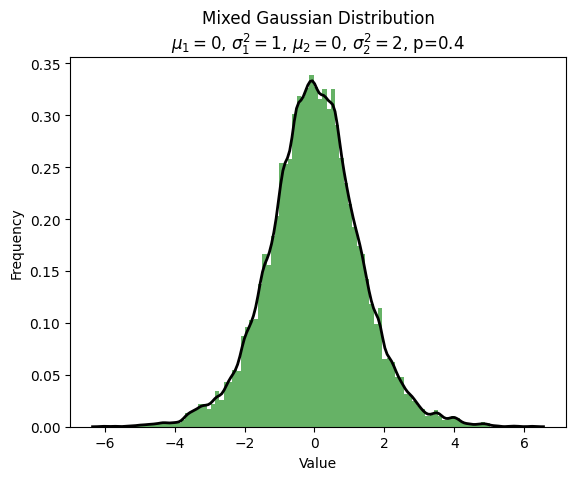
\includegraphics[width=\linewidth]{figure/mu_2=0.png}
        \caption{$\mu_2=0$}
    \end{minipage}
    \hfill
    \begin{minipage}[b]{0.2\linewidth}
        \centering
        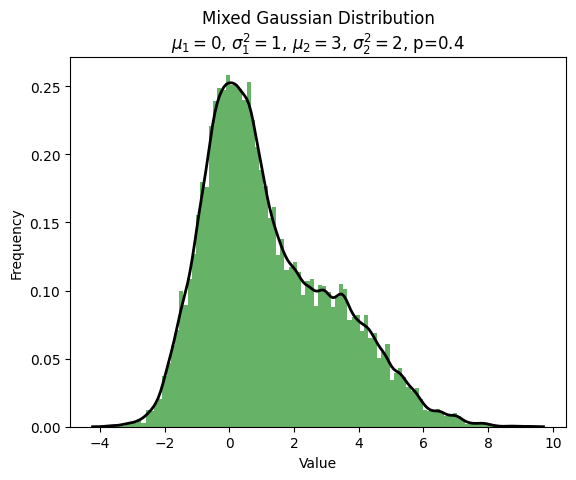
\includegraphics[width=\linewidth]{figure/mu_2=3.png}
        \caption{$\mu_2=3$}
    \end{minipage}
    \hfill
    \begin{minipage}[b]{0.2\linewidth}
        \centering
        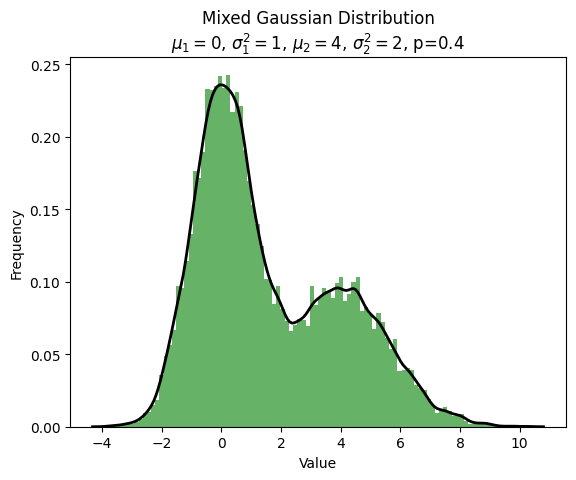
\includegraphics[width=\linewidth]{figure/mu_2=4.png}
        \caption{$\mu_2=4$}
    \end{minipage}
    \hfill
    \begin{minipage}[b]{0.2\linewidth}
        \centering
        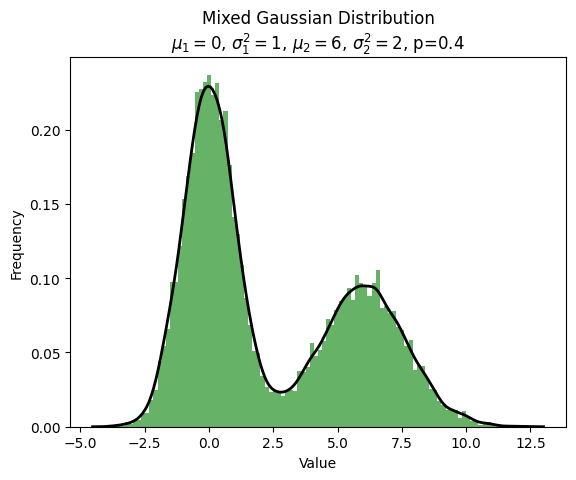
\includegraphics[width=\linewidth]{figure/mu_2=6.png}
        \caption{$\mu_2=6$}
    \end{minipage}
    \caption{$\mu_2$对“峰”的影响}
    \label{fig:mu_2递增}
\end{figure}

\subsubsection{\texorpdfstring{$\sigma_2^2$对“峰”的影响}{sigma2平方对“峰”的影响}}

控制其它参数不变,改变$\sigma_2^2$的值,绘制出如下图\ref{fig:sigma_2}所示的一组图片。

\begin{figure}[H]
    \centering
    \begin{minipage}[b]{0.3\linewidth}
        \centering
        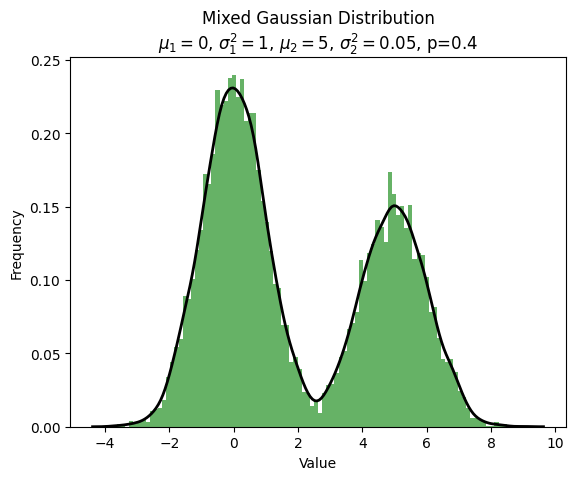
\includegraphics[width=\linewidth]{figure/sigma_^2=0.05.png}
        \caption{$\sigma_2^2=0.05$}
    \end{minipage}
    \hfill
    \begin{minipage}[b]{0.3\linewidth}
        \centering
        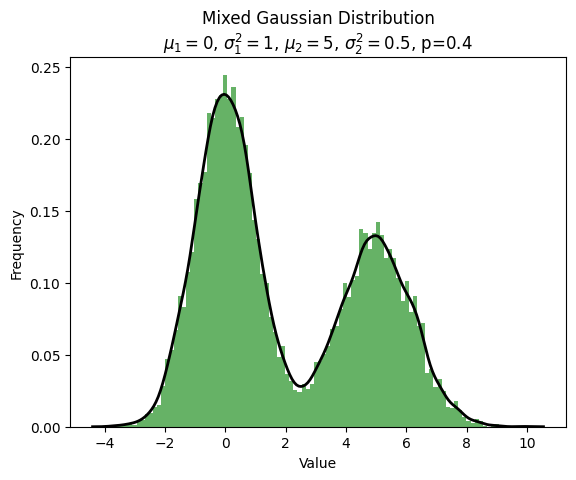
\includegraphics[width=\linewidth]{figure/sigma_^2=0.5.png}
        \caption{$\sigma_2^2=0.5$}
    \end{minipage}
    \hfill
    \begin{minipage}[b]{0.3\linewidth}
        \centering
        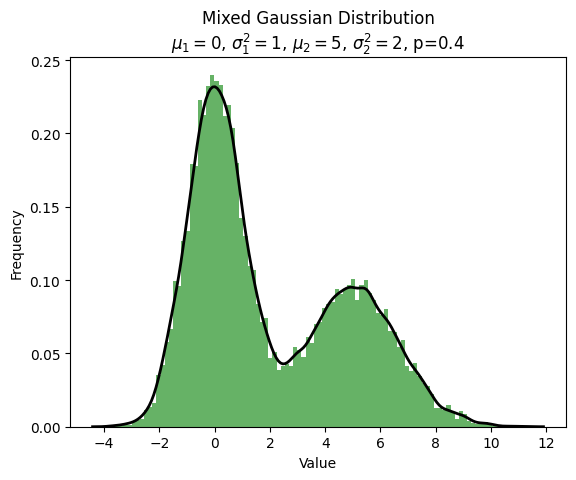
\includegraphics[width=\linewidth]{figure/sigma_^2=2.png}
        \caption{$\sigma_2^2=2$}
    \end{minipage}
    \vspace{4mm} % 控制上下图片间的间隔
    \begin{minipage}[b]{0.3\linewidth}
        \centering
        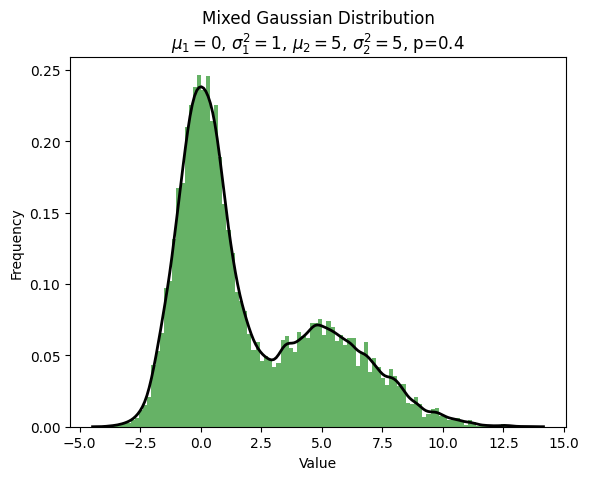
\includegraphics[width=\linewidth]{figure/sigma_^2=5.png}
        \caption{$\sigma_2^2=5$}
    \end{minipage}
    \hfill
    \begin{minipage}[b]{0.3\linewidth}
        \centering
        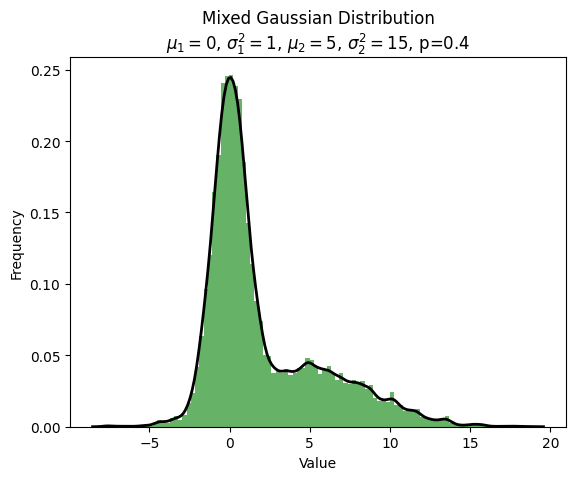
\includegraphics[width=\linewidth]{figure/sigma_^2=15.png}
        \caption{$\sigma_2^2=15$}
    \end{minipage}
    \hfill
    \begin{minipage}[b]{0.3\linewidth}
        \centering
        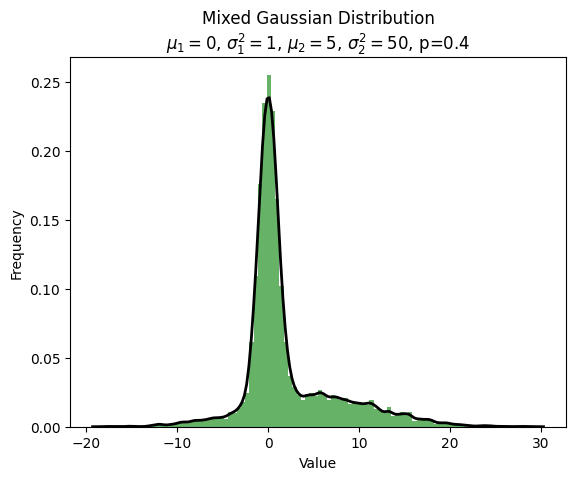
\includegraphics[width=\linewidth]{figure/sigma_^2=50.png}
        \caption{$\sigma_2^2 =50$}
    \end{minipage}
    \caption{$\sigma_2^2$对“峰”的影响}
    \label{fig:sigma_2}
\end{figure}

通过对图中数据的仔细观察,我们可以发现$\sigma_2^2$对主峰的特征没有显著影响。然而,次峰的高度和陡峭程度明显依赖于$\sigma_2^2$的大小。随着$\sigma_2^2$的增加,次峰的高度逐渐降低,并且其周边变得更加平缓。当$\sigma_2^2$达到一定阈值后,次峰变得难以辨识。这些观察使我们可以合理推测,$\sigma_2^2$对次峰的形态特征具有显著影响。\label{sec:peak_influence}

\subsubsection{\texorpdfstring{$p$对“峰”的影响}{p对“峰”的影响}}

控制其它参数不变,逐步改变$p$的值,绘制出如下图\ref{fig:p}所示的一组图片。

\begin{figure}[H]
    \centering
    \begin{minipage}[b]{0.3\linewidth}
        \centering
        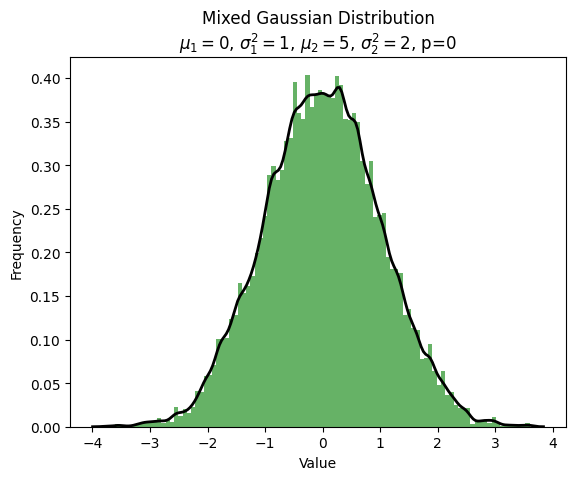
\includegraphics[width=\linewidth]{figure/p=0.png}
        \caption{$p=0$}
    \end{minipage}
    \hfill
    \begin{minipage}[b]{0.3\linewidth}
        \centering
        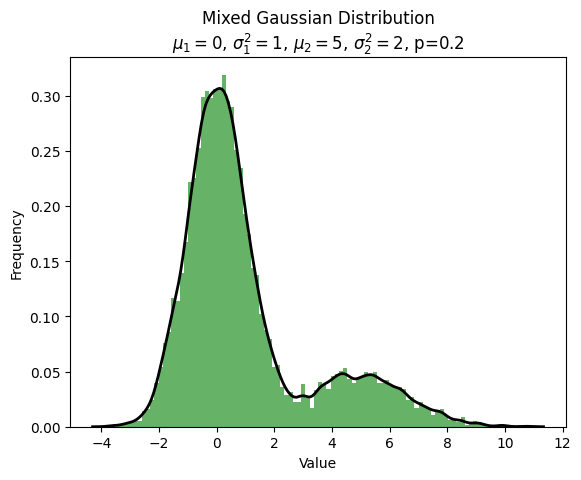
\includegraphics[width=\linewidth]{figure/p=0.2.png}
        \caption{$p=0.2$}
    \end{minipage}
    \hfill
    \begin{minipage}[b]{0.3\linewidth}
        \centering
        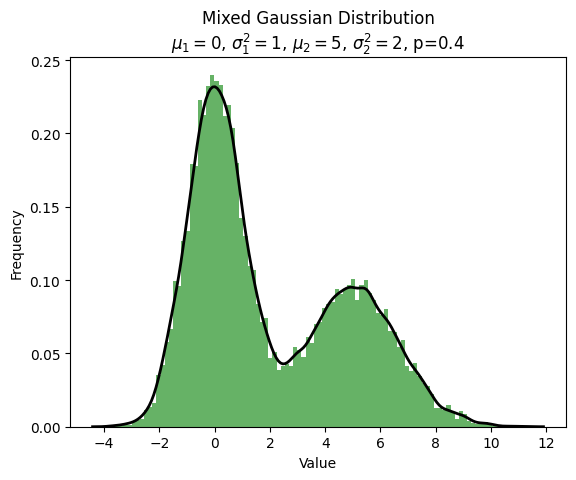
\includegraphics[width=\linewidth]{figure/p=0.4.png}
        \caption{$p=0.4$}
    \end{minipage}
    \vspace{4mm} % 控制上下图片间的间隔
    \begin{minipage}[b]{0.3\linewidth}
        \centering
        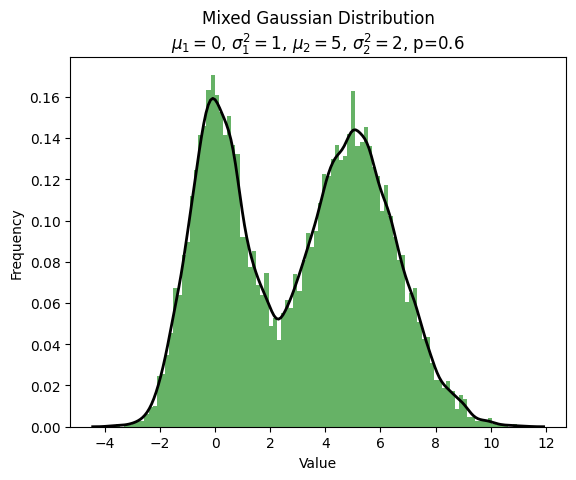
\includegraphics[width=\linewidth]{figure/p=0.6.png}
        \caption{$p=0.6$}
    \end{minipage}
    \hfill
    \begin{minipage}[b]{0.3\linewidth}
        \centering
        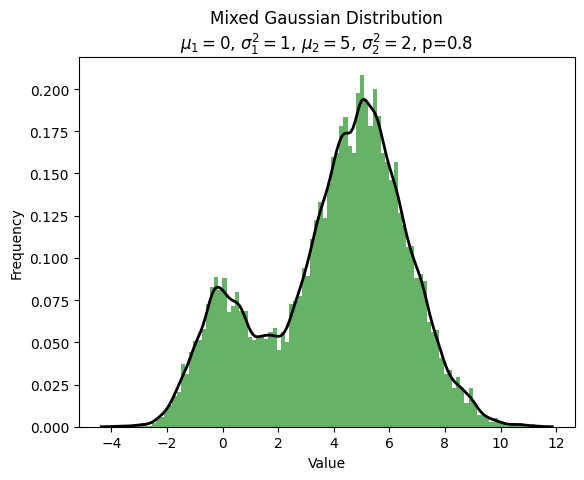
\includegraphics[width=\linewidth]{figure/p=0.8.png}
        \caption{$p=0.8$}
    \end{minipage}
    \hfill
    \begin{minipage}[b]{0.3\linewidth}
        \centering
        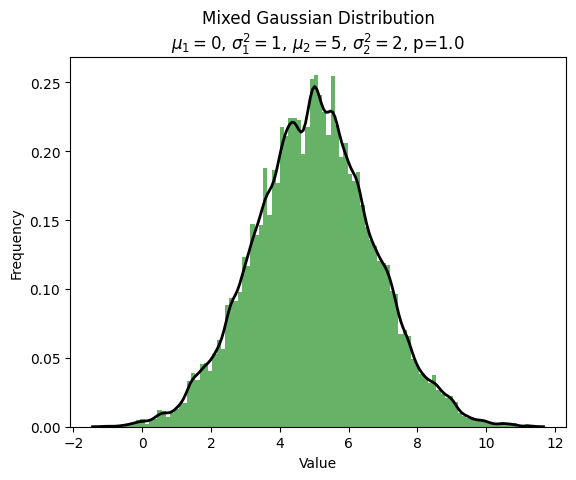
\includegraphics[width=\linewidth]{figure/p=1.0.png}
        \caption{$p=1.0$}
    \end{minipage}
    \caption{$p$对“峰”的影响}
    \label{fig:p}
\end{figure}

在上述图片中,本文通过逐渐调整第二高斯分量的权重参数 \( p \) 从 0 到 1.0,观察到分布形态的显著变化。最初,分布完全由第一个高斯分量控制,表现为一个集中在 \( \mu_1 \) 的单一峰,即一个标准正态分布的形状。随着 \( p \) 的增加,第二分量逐渐显示出其影响力,导致峰值从 \( \mu_1 \) 向 \( \mu_2 = 5 \) 移动,直至 \( p = 1.0 \) 时由 \( \mu_2 \) 和 \( \mu_2 \)共同主导,表现为两个正态分布加和的图像。这一过程中,\( \mu_1 \) 附近的主峰逐渐降低,而 \( \mu_2 \) 附近的峰则逐步增高并变得更加显著,当$p$接近某一值时,会出现两峰高度相同的情况。\label{sec:p}

\subsubsection{\texorpdfstring{$\mu_1$对“峰”的影响}{mu1对“峰”的影响}}

控制其它参数不变,仅改变$\mu_1$的值,绘制出如图\ref{fig:mu1}一组图片。

\begin{figure}[H]
    \centering
    \begin{minipage}[b]{0.3\linewidth}
        \centering
        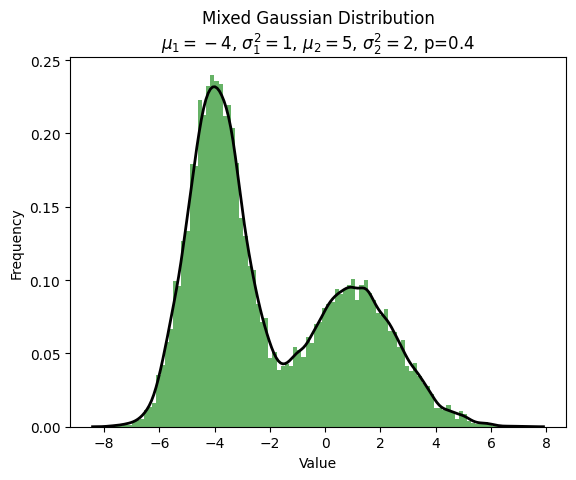
\includegraphics[width=\linewidth]{figure/mu_1=-4.png}
        \caption{$\mu_1=-4$}
    \end{minipage}
    \hfill
    \begin{minipage}[b]{0.3\linewidth}
        \centering
        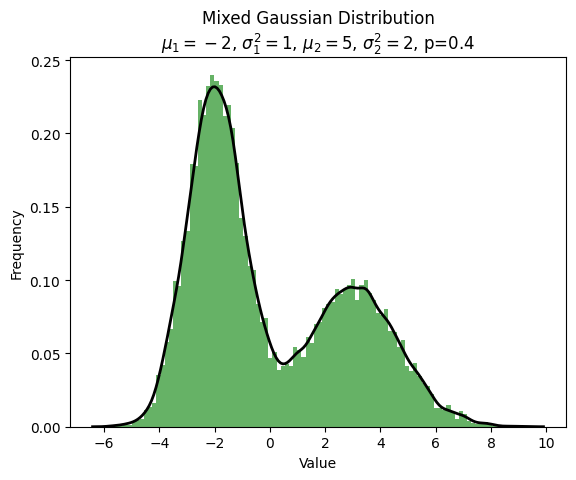
\includegraphics[width=\linewidth]{figure/mu_1=-2.png}
        \caption{$\mu_1=-2$}
    \end{minipage}
    \hfill
    \begin{minipage}[b]{0.3\linewidth}
        \centering
        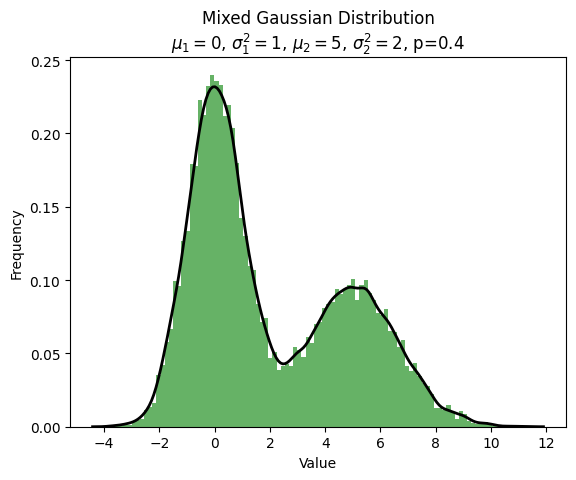
\includegraphics[width=\linewidth]{figure/mu_1=0.png}
        \caption{$\mu_1=0$}
    \end{minipage}
    \vspace{4mm} % 控制上下图片间的间隔
    \begin{minipage}[b]{0.3\linewidth}
        \centering
        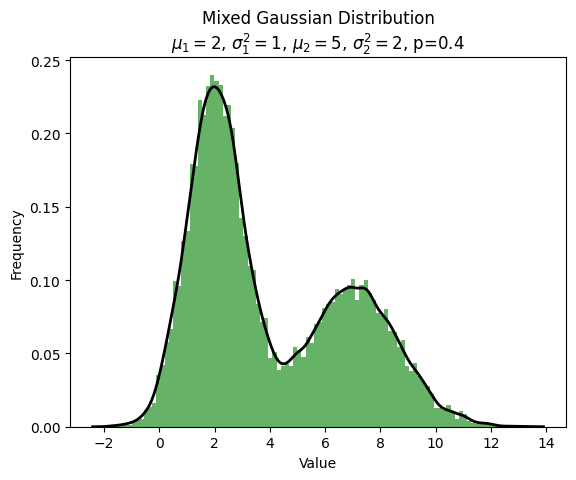
\includegraphics[width=\linewidth]{figure/mu_1=2.png}
        \caption{$\mu_1=2$}
    \end{minipage}
    \hfill
    \begin{minipage}[b]{0.3\linewidth}
        \centering
        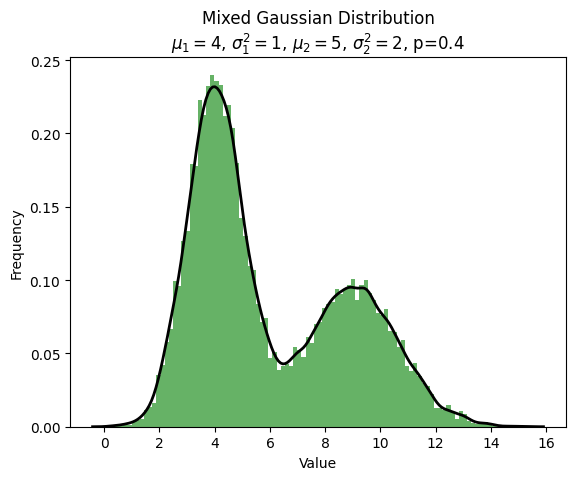
\includegraphics[width=\linewidth]{figure/mu_1=4.png}
        \caption{$\mu_1=4$}
    \end{minipage}
    \hfill
    \begin{minipage}[b]{0.3\linewidth}
        \centering
        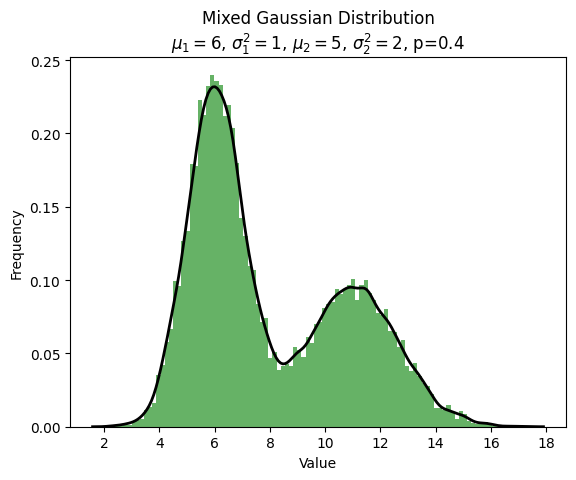
\includegraphics[width=\linewidth]{figure/mu_1=6.png}
        \caption{$\mu_1=6$}
    \end{minipage}
    \caption{$\mu_1$对“峰”的影响}
    \label{fig:mu1}
\end{figure}

观察这组图片可以发现,混合高斯分布频率分布直方图的形状并没有发生改变,改变$\mu_1$的结果表现为图像整体在水平方向上的平移,平移量即为$\mu_1$的该变量。\label{sec:mu1}

\subsubsection{\texorpdfstring{$\sigma_1^2$对“峰”的影响}{sigma1平方对“峰”的影响}}

控制其它参数不变,仅改变$\sigma_1^2$的值,绘制出如图\ref{fig:sigma1}一组图片。

\begin{figure}[H]
    \centering
    \begin{minipage}[b]{0.3\linewidth}
        \centering
        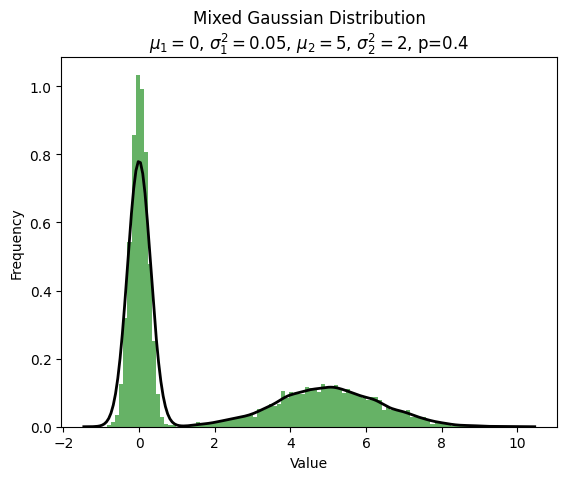
\includegraphics[width=\linewidth]{figure/sigma_1^2=0.05.png}
        \caption{$\sigma_1^2=0.05$}
    \end{minipage}
    \hfill
    \begin{minipage}[b]{0.3\linewidth}
        \centering
        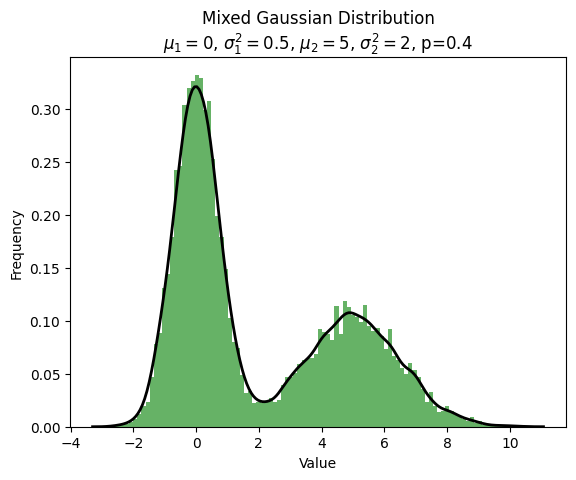
\includegraphics[width=\linewidth]{figure/sigma_1^2=0.5.png}
        \caption{$\sigma_1^2=0.5$}
    \end{minipage}
    \hfill
    \begin{minipage}[b]{0.3\linewidth}
        \centering
        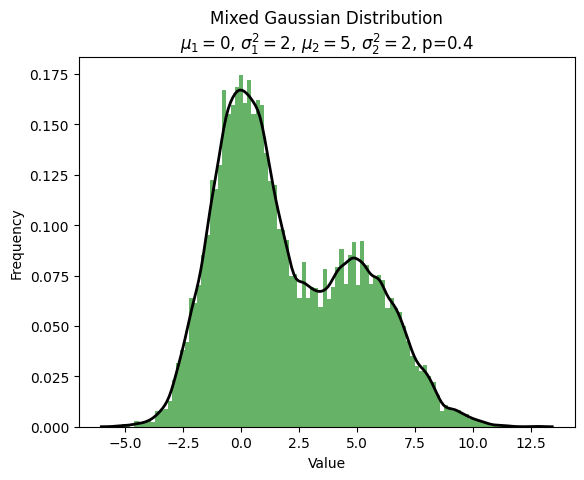
\includegraphics[width=\linewidth]{figure/sigma_1^2=2.png}
        \caption{$\sigma_1^2=2$}
    \end{minipage}
    \vspace{4mm} % 控制上下图片间的间隔
    \begin{minipage}[b]{0.3\linewidth}
        \centering
        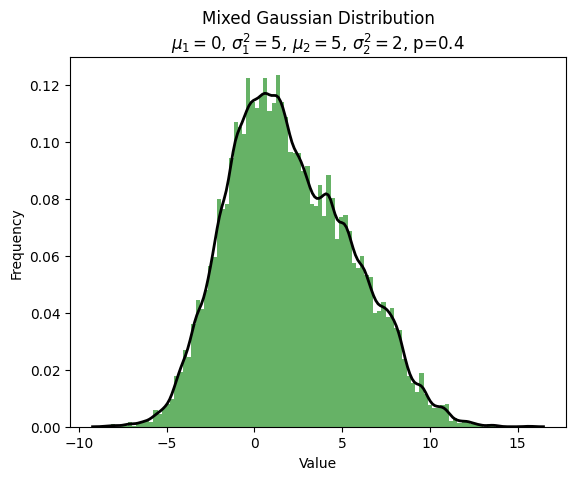
\includegraphics[width=\linewidth]{figure/sigma_1^2=5.png}
        \caption{$\sigma_1^2=5$}
    \end{minipage}
    \hfill
    \begin{minipage}[b]{0.3\linewidth}
        \centering
        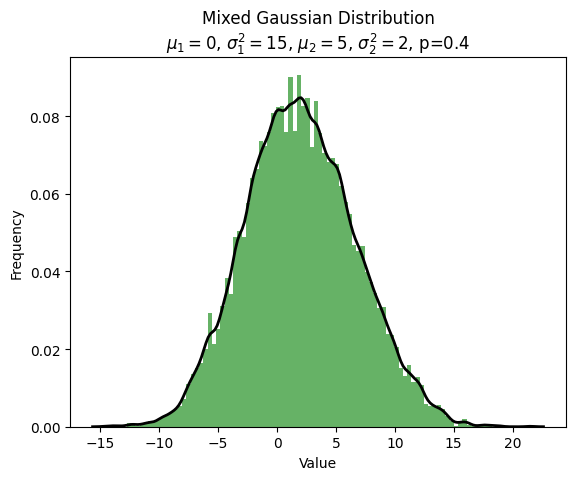
\includegraphics[width=\linewidth]{figure/sigma_1^2=15.png}
        \caption{$\sigma_1^2=15$}
    \end{minipage}
    \hfill
    \begin{minipage}[b]{0.3\linewidth}
        \centering
        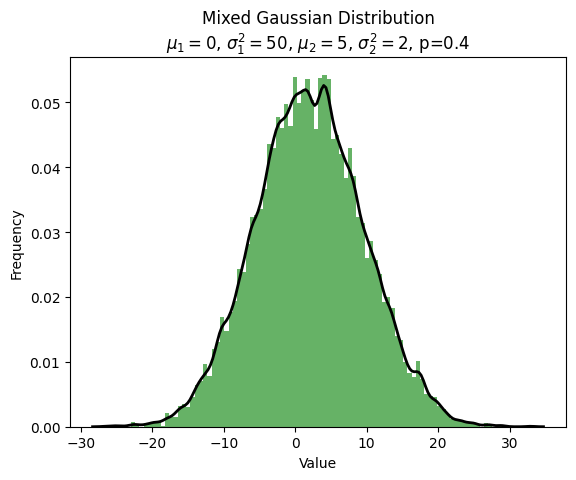
\includegraphics[width=\linewidth]{figure/sigma_1^2=50.png}
        \caption{$\sigma_1^2=50$}
    \end{minipage}
    \caption{$\sigma_1^2$对“峰”的影响}
    \label{fig:sigma1}
\end{figure}

通过观察这组图像,可以发现方差 $\sigma_1^2$ 对主峰的影响与方差 $\sigma_2^2$ 对次峰的影响具有一定的相似性。随着 $\sigma_1^2$ 的增加,主峰的高度逐渐降低,峰形也变得更加平缓。当 $\sigma_1^2$ 达到一定的值时,主峰变得难以辨识。为了与 $\sigma_2^2$ 对次峰的影响进行比较,本实验中 $\sigma_1^2$ 的变化范围与 $\sigma_2^2$ 的变化范围保持一致。结果表明,$\sigma_1^2$ 对主峰的影响比 $\sigma_2^2$ 对次峰的影响显著更为剧烈。\label{sec:sigma1}

\subsection{利用混合高斯分布的密度函数解释上述现象}

\subsubsection{混合高斯分布密度函数推导}

考虑随机变量 \( X \sim \mathcal{N}(\mu_1, \sigma_1^2) \),\( Y \sim \mathcal{N}(\mu_2, \sigma_2^2) \),以及 \( Z = X + \eta Y \),其中 \( P(\eta = 0) = p \),\( P(\eta = 1) = 1 - p \),且 \( \eta \) 与 \( X \)、\( Y \) 相互独立。由此可以推得:

\[
X + Y \sim \mathcal{N}(\mu_1 + \mu_2, \sigma_1^2 + \sigma_2^2)
\]

接下来我们推导混合高斯分布的累积分布函数(CDF)。首先,混合高斯分布的累积分布函数 \( F_Z(z) \) 为:

\begin{equation}
F_Z(z) = P(Z \leq z) = P(X + \eta Y \leq z)
\end{equation}

由于 \( \eta \) 取值为 0 或 1,我们可以展开:

\begin{equation}
F_Z(z) = P(X \leq z | \eta = 0) P(\eta = 0) + P(X + Y \leq z | \eta = 1) P(\eta = 1)
\end{equation}

进一步代入 \( P(\eta = 0) = 1 - p \) 和 \( P(\eta = 1) = p \),我们得到:

\begin{equation}
F_Z(z) = (1 - p) \int_{-\infty}^z \frac{1}{\sqrt{2\pi} \sigma_1} e^{-\frac{(x - \mu_1)^2}{2 \sigma_1^2}} \, dx + p \int_{-\infty}^z \frac{1}{\sqrt{2\pi} \sqrt{\sigma_1^2 + \sigma_2^2}} e^{-\frac{(x - \mu_1 - \mu_2)^2}{2(\sigma_1^2 + \sigma_2^2)}} \, dx
\label{eq1}
\end{equation}

对上式求导,即可得到密度函数 \( f_Z(z) \):

\begin{equation}
f_Z(z) = (1 - p) \frac{1}{\sqrt{2\pi} \sigma_1} e^{-\frac{(z - \mu_1)^2}{2 \sigma_1^2}} + p \frac{1}{\sqrt{2\pi} \sqrt{\sigma_1^2 + \sigma_2^2}} e^{-\frac{(z - \mu_1 - \mu_2)^2}{2 (\sigma_1^2 + \sigma_2^2)}}
\label{eq2}
\end{equation}

\subsubsection{密度函数对前文推测的解释}

通过分析混合高斯分布的密度函数\ref{eq2}可以得出以下结论:

\begin{enumerate}
  \item 增大 \( \mu_2 \) 会使两个峰之间的间距增大,这与\ref{sec:peak_dist}中的结果一致。而 \( \mu_1 \) 的变化则会使两个峰平移相同的距离,这与\ref{sec:mu1}中的结论相符。从密度函数的角度来看,混合高斯分布的对称性取决于 \( \mu_1 \) 和 \( \mu_2 \) 的相对位置。当 \( \mu_1 = 0 \) 且 \( \mu_2 \) 关于 \( \mu_1 \) 对称时,密度函数中的两个峰分别位于 0 和 \( \mu_2 \) 处。在这种情况下,若 \( \mu_2 \) 相对于 \( \mu_1 \) 对称,两个峰的位置和形状将保持一致,从而使混合高斯分布呈现出明显的对称性。然而,当 \( \mu_1 \neq 0 \) 时,即使 \( \mu_2 \) 相对于 \( \mu_1 \) 对称,密度函数的两个峰分别位于 \( \mu_1 \) 和 \( \mu_1 + \mu_2 \) 处。此时,因 \( \mu_1 \) 的偏移,两个峰之间的距离会减小,且出现“挤压”现象,导致分布的整体对称性减弱。这一现象验证了\ref{sec:symmetry}中的观察结果。
  \item \( \sigma_1^2 \) 和 \( \sigma_2^2 \) 的变化影响了峰的形状。当方差增大时,两个峰的高度会降低,且形状变得更加平缓。尤其是由于 \( \sigma_1^2 \) 同时作用于密度函数的两项,这使得 \( \sigma_1^2 \) 的变化对分布的影响更加显著,验证了\ref{sec:sigma1}和\ref{sec:peak_influence}中的结论。
  \item \( p \) 代表两个高斯分布的权重,通过调整 \( p \) 的值可以改变两个峰的相对高度。当 \( p \) 增大时,次峰相对于主峰的高度也随之增大。在密度函数中,权重较大的那一项对应的峰会更加明显,这一现象验证了\ref{sec:p}中的结论。
\end{enumerate}

\section{任务二}

\subsection{混合高斯分布的期望与方差推导}

由$X$、$Y$、$\eta$独立,可由下面的式子得出混合高斯分布的期望与方差:

\textbf{1. 期望 $E(Z)$:}
\[
E(Z) = E(X + \eta Y) = E(X) + E(\eta)E(Y) = \mu_1 + p \mu_2
\]

\textbf{2. 方差 $D(Z)$:}
\[
D(Z) = D(X + \eta Y) = D(X) + D(\eta Y)
\]
又
\[
D(\eta Y) = E(\eta^2 Y^2) - E^2(\eta Y)
\]
\[
E(\eta^2 Y^2) = E(\eta^2)E(Y^2), \quad E(\eta Y) = E(\eta)E(Y)
\]
因此,
\[
D(\eta Y) = E(\eta^2)E(Y^2) - (E(\eta)E(Y))^2
\]
\[
= (E^2(\eta) + D(\eta))(E^2(Y) + D(Y)) - (E(\eta)E(Y))^2
\]
\[
= E^2(\eta)D(Y) + E^2(Y)D(\eta) + D(\eta)D(Y)
\]
从而,
\[
D(Z) = \sigma_1^2 + p \sigma_2^2 + \mu_2^2 p (1 - p)
\]

\subsection{随机变量$U$的频率分布直方图及样本量$n$对其峰的影响}

\subsubsection{\texorpdfstring{随机变量$U$的定义及其含义}{随机变量U的定义及其含义}}

统计量 $U$ 的定义为:
\begin{equation}
U_i = \frac{1}{\sqrt{n \text{Var}(Z)}} \left( \sum_{j=1}^n Z_{i,j} - n \mathbb{E}[Z] \right)
\label{eq3}
\end{equation}
其中 $Z_{i,j}$ 是从混合高斯分布中独立抽样得到的随机变量。

观察定义式\ref{eq3},可以得到$U_i$实际上为n个共同分布为混合高斯分布的独立同分布随机变量之和并标准化后的结果。

为使其频率分布直方图特性鲜明,此处采用$\mu_1=0$、$\sigma_1^2=1$、$\mu_2=20$、$\sigma_2^2=0.1$、$p=0.4$,对$n=2,3,4,5,10,20,50,1000,5000$分别采样1000组,并绘制如下频率分布直方图。

\subsubsection{\texorpdfstring{随机变量$U$的频率分布直方图}{随机变量U的频率分布直方图}}

\begin{figure}[H]
    \centering
    \begin{minipage}[b]{0.3\linewidth}
        \centering
        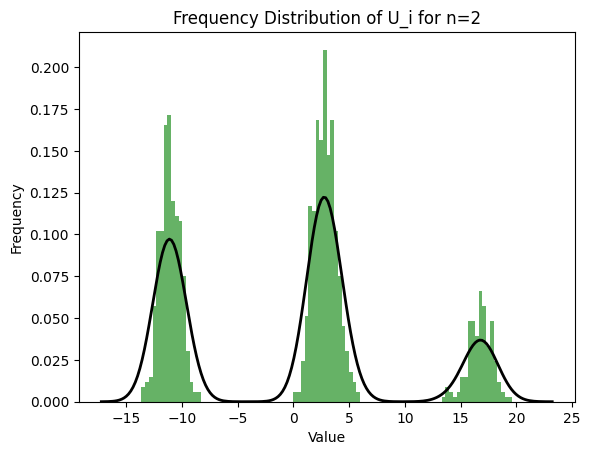
\includegraphics[width=\linewidth]{figure/n=2.png}
        \caption{$n=2$}
    \end{minipage}
    \hfill
    \begin{minipage}[b]{0.3\linewidth}
        \centering
        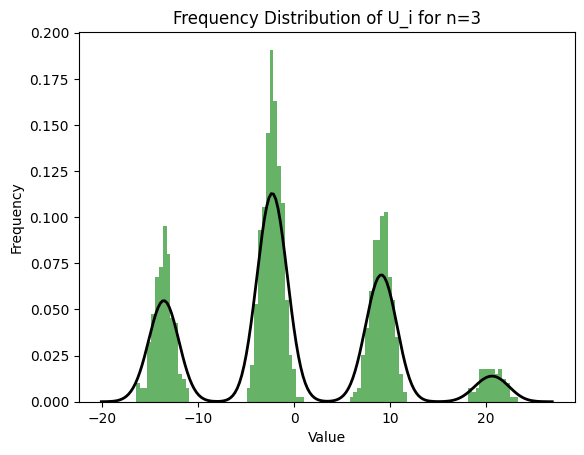
\includegraphics[width=\linewidth]{figure/n=3.png}
        \caption{$n=3$}
    \end{minipage}
    \hfill
    \begin{minipage}[b]{0.3\linewidth}
        \centering
        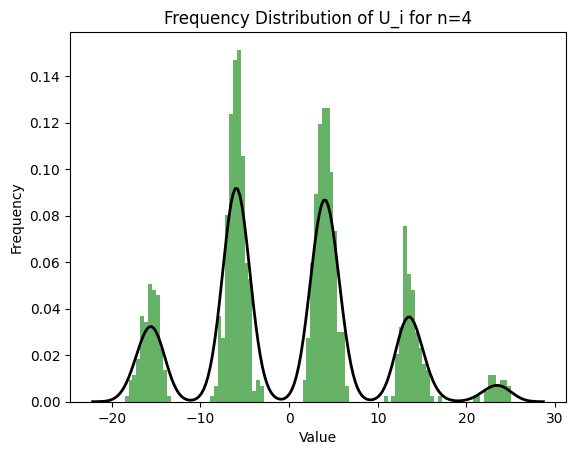
\includegraphics[width=\linewidth]{figure/n=4.png}
        \caption{$n=4$}
    \end{minipage}
    \vspace{4mm} % 控制上下图片间的间隔
    \begin{minipage}[b]{0.3\linewidth}
        \centering
        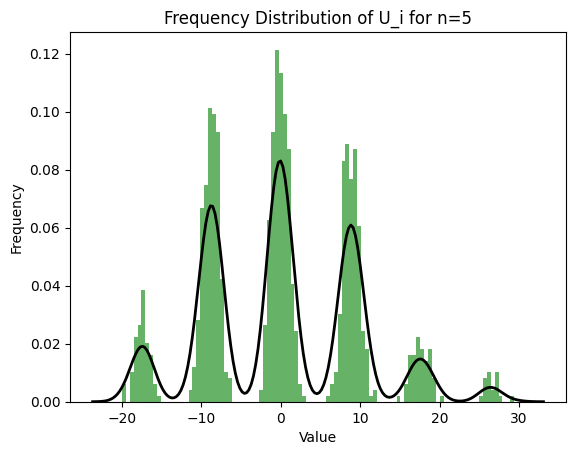
\includegraphics[width=\linewidth]{figure/n=5.png}
        \caption{$n=5$}
    \end{minipage}
    \hfill
    \begin{minipage}[b]{0.3\linewidth}
        \centering
        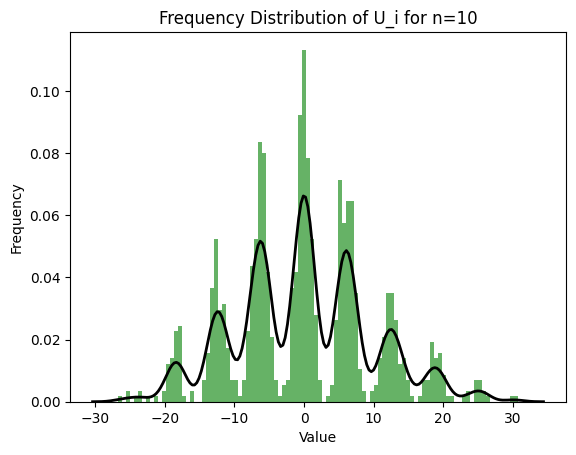
\includegraphics[width=\linewidth]{figure/n=10.png}
        \caption{$n=10$}
    \end{minipage}
    \hfill
    \begin{minipage}[b]{0.3\linewidth}
        \centering
        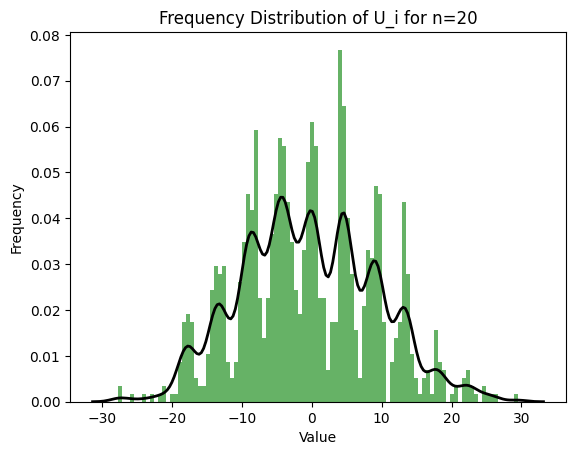
\includegraphics[width=\linewidth]{figure/n=20.png}
        \caption{$n=20$}
    \end{minipage}
    \vspace{4mm} % 控制上下图片间的间隔
    \begin{minipage}[b]{0.3\linewidth}
        \centering
        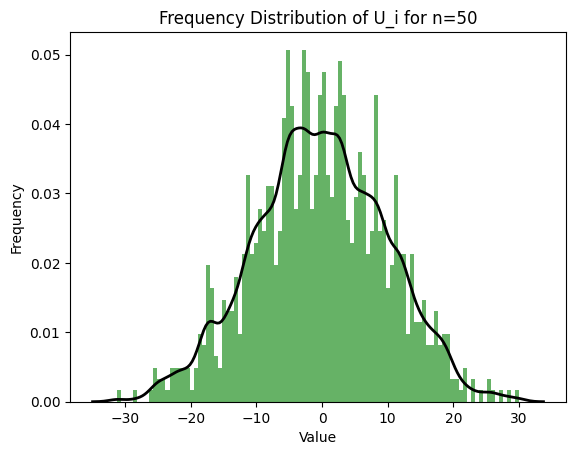
\includegraphics[width=\linewidth]{figure/n=50.png}
        \caption{$n=50$}
    \end{minipage}
    \hfill
    \begin{minipage}[b]{0.3\linewidth}
        \centering
        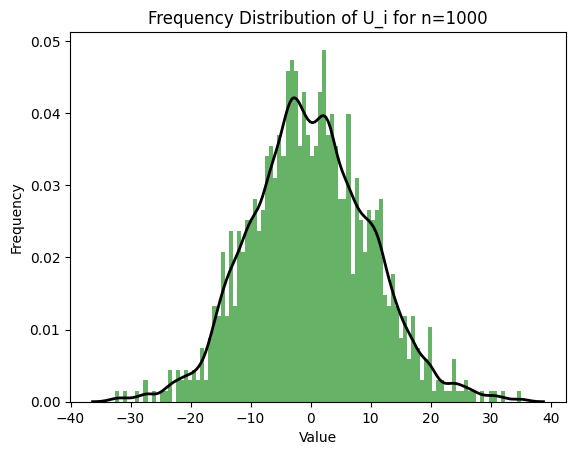
\includegraphics[width=\linewidth]{figure/n=1000.png}
        \caption{$n=1000$}
    \end{minipage}
    \hfill
    \begin{minipage}[b]{0.3\linewidth}
        \centering
        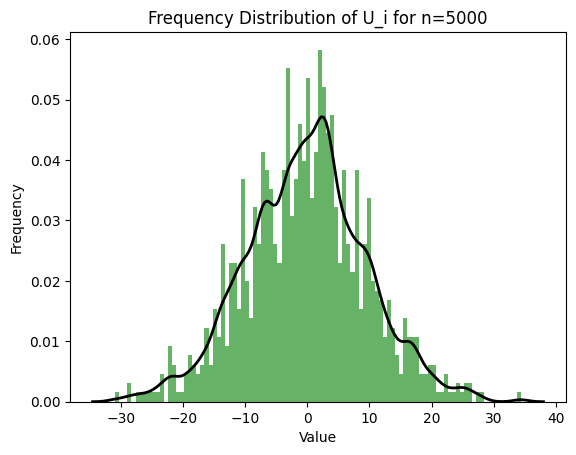
\includegraphics[width=\linewidth]{figure/n=5000.png}
        \caption{$n=5000$}
    \end{minipage}
    \caption{$n$对“峰”的影响}
    \label{fig:n}
\end{figure}

观察这组图片可以发现,随着$n$的增大,“峰”的个数在逐渐增多,$n$较小时,“峰“的个数约为$n+1$个;但当$n$足够大时,“峰”的个数逐渐变为一个。

\subsubsection{理论分析}

首先我们推导混合高斯分布的矩母函数 \( M_Z(t) \) :
\[
M_Z(t) = (1-p) \exp\left(t \mu_1 + \frac{t^2}{2} \sigma_1^2\right) + p \exp\left(t(\mu_1 + \eta \mu_2) + \frac{t^2}{2}(\sigma_1^2 + \eta^2 \sigma_2^2)\right).
\]

计算 \( \mathbb{E}[e^{tU}] \),即 \( U_i \) 的矩母函数 \( M_U(t) \):

\[
M_U(t) = \mathbb{E}\left[ \exp\left(t \cdot \frac{1}{\sqrt{n \text{Var}(Z)}} \left( \sum_{j=1}^n Z_{i,j} - n \mathbb{E}[Z] \right) \right) \right].
\]

这里 \( \sum_{j=1}^n Z_{i,j} \) 是从混合高斯分布中抽取的 \( n \) 个样本的和,且由于这些样本是独立同分布的,我们有:
\[
\mathbb{E}\left[ \exp\left(t \cdot \frac{1}{\sqrt{n \text{Var}(Z)}} \left( \sum_{j=1}^n Z_{i,j} - n \mathbb{E}[Z] \right) \right) \right] = \prod_{j=1}^n \mathbb{E}\left[ \exp\left( t \cdot \frac{1}{\sqrt{n \text{Var}(Z)}} \left(Z_{i,j} - \mathbb{E}[Z]\right) \right) \right].
\]

注意到 \( Z_{i,j} - \mathbb{E}[Z] \) 是零均值的混合高斯分布随机变量。

对每个单独的随机变量 \( Z_{i,j} \),我们有:
\[
\mathbb{E}\left[ \exp\left( t \cdot \frac{1}{\sqrt{n \text{Var}(Z)}} \left( Z_{i,j} - \mathbb{E}[Z] \right) \right) \right] = \exp\left( - \frac{t^2}{2n \text{Var}(Z)} \right).
\]

因为 \( Z_{i,j} \) 来自混合高斯分布,这个期望值将由两个高斯成分的加权平均组成:

\[
M_{Z_{i,j} - \mathbb{E}[Z]}(t) = (1-p) \exp\left( -\frac{t^2}{2n \sigma_1^2} \right) + p \exp\left( -\frac{t^2}{2n (\sigma_1^2 + \eta^2 \sigma_2^2)} \right).
\]

因此,\( U_i \) 的矩母函数为:

\begin{equation}
M_U(t) = \left[ (1-p) \exp\left( -\frac{t^2}{2n \sigma_1^2} \right) + p \exp\left( -\frac{t^2}{2n (\sigma_1^2 + \eta^2 \sigma_2^2)} \right) \right]^n.
\label{eq4}
\end{equation}

下面利用式\ref{eq4}解释频率分布直方图中“峰”受n影响而产生的变化:

\begin{itemize}
    \item 当 \( n \) 较小时,由于样本均值 \( \sum_{j=1}^n Z_{i,j} \) 还没有完全收敛于理论期望 \( \mathbb{E}[Z] \),统计量 \( U_i \) 受到混合分布的影响。因为混合分布有两个成分,\( U_i \) 的分布在有限样本时表现出多个峰值。
    \item \textbf{为什么会有多个峰?}
    \begin{itemize}
        \item 每个样本的值 \( Z_{i,j} \) 可能来自两个不同的高斯成分。由于 \( Z_{i,j} \) 的期望不同,样本均值可能集中在不同的区域,这些区域对应于混合分布中的不同高斯成分。
        \item 由于统计量 \( U_i \) 是样本均值的标准化形式,它反映了这些区域的偏差。每个高斯成分的样本均值会贡献一个峰值。
        \item 因此,在有限样本的情况下,矩母函数的结果是一个多峰分布,其峰的数量大致与混合分布成分的数量相关,即大约有 \( n+1 \) 个峰。
        \item 当样本量足够大时,样本均值趋向于 \( \mathbb{E}[Z] \),矩母函数逐渐趋近于标准正态分布,从而消除了多峰现象,分布服从独立同分布的中心极限定理,呈现单峰的正态分布。
    \end{itemize}
\end{itemize}


\section{感想}

行文至此,概率论这门课的大作业终于圆满完成。尽管不至于历经艰险,却也经历了一些曲折。从课堂上初识混合高斯分布,到逐步理解并拆解任务,从敲下第一行代码,到完成所有绘图,从查阅资料、向学长求教,到最终完成理论分析,每一步都凝聚着努力与收获。完成这份大作业后,我不仅对高斯分布这一被称为“世界最重要分布”的理解更加深入,也对概率论中的公式、定理与分布有了更加具象的体悟,同时也极大地提升了自学能力。

关于这门课,我感触良多。学期初,或许是因为刚学完概统,再加上作为双学位学生,本学期的经济学课程也涉及了不少概率统计相关内容,我一度觉得概率论与概率统计的前半部分非常相似,只是在定义上借助测度论做了延拓,而实际应用部分却并无太大差异。然而,涉及测度论的部分对我来说相对陌生且艰深,起初让我对这门课的热情有所减退。但随着课程的推进,我逐渐意识到,事实并非如此。概率论不仅探讨了许多概率统计中浅尝辄止的知识点,还涵盖了自身独特的内容,例如各种收敛性以及更复杂、更贴近现实的分布。熊老师通过现实案例引入教学内容,让我切实感受到概率论在实际生活中的广泛应用。这些体验让我逐步领悟到,概率论的价值不仅仅体现在学科间的丰富应用,更在于它能够体系化地解释真实世界中的不确定性。

在此,我衷心感谢熊老师为我们提供了这样一个难得的机会,既加深了我们对概率论的理解,也锻炼了我们的多方面能力。同时,也感谢熊老师在整个学期中的辛勤付出和耐心教学,感谢助教们的悉心批改与答疑。特别感谢谭宇学长对我的指点,他的指导让我初步掌握了矩母函数的相关知识,并成功将其应用于任务二的分析中。希望这种有趣且富有实际意义的大作业能够继续传承,让更多同学受益。

再次致以诚挚的感谢!

\newpage

\begin{appendices}
\section{Python Code}
以下是用于完成本次作业的 Python 代码:

\lstinputlisting[caption={混合高斯分布频率直方图生成代码}, label={lst:python-code}]{code/task1.py}

\newpage

\lstinputlisting[caption={随机变量 U 频率直方图生成代码}, label={lst:python-code}]{code/task2.py}

\end{appendices}

\end{document}
